\section{Overview}\label{sec:impl-overview}

\iblock{} is developed in C++23 on top of the \omnetpp{} discrete-event
simulation framework (see \secref{sec:omnetpp}) and is compatible with
\omnetpp{} version 6.x.

An \iblock{} network consists of multiple nodes that communicate through
\emph{direct messages} rater than traditional \omnetpp{} links.
\figref{fig:iblock-network} shows an example of a 10-node network in the
\omnetpp{}'s QT environment.

\begin{figure}[tbhp]
	\centering
	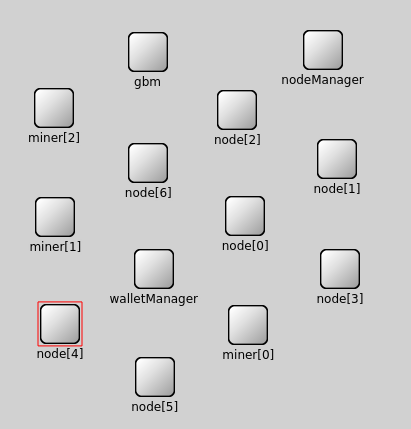
\includegraphics[width=0.5\textwidth]{iblock-qt-network}
	\caption{An \iblock{} network in the OMNeT++'s QT
	environment.}\label{fig:iblock-network}
\end{figure}

Nodes in \iblock{} can vary by type and be configured with different
parameters, utilizing the flexibility of \omnetpp{}'s configuration
capabilities. In \figref{fig:iblock-network}, two primary types of nodes
are visible: \emph{Miner} nodes and \emph{User} nodes (labeled as ``node[*]'').
\emph{Miner} contain a \emph{Miner application} capable of mining blocks and
earning rewards, while \emph{User} nodes feature a \emph{TransactionGenerator
application} to create and submit transactions to the network.

The network also includes special-purpose module:
\begin{itemize}
	\item The \code{gbm} (Global Blockchain Manager) module creates the
		\emph{genesis block} at startup and manages memory by removing
		unneeded blocks;
	\item The \code{walletManager} module acts as a directory for other
		nodes to retrieve wallet addresses;
	\item The \code{nodeManager} module serves as a directory for all nodes
		in the network, allowing nodes to request references for
		message sending.
\end{itemize}

Each of these special-purpose modules is detailed further in
\secref{sec:impl-global}.

As previously noted, the network omits typical links between nodes. Instead,
node-to-node communication is facilitated by \emph{direct messages} using
\omnetpp{}'s \code{sendDirect()} function. Communication between nodes and
global modules is handled via \emph{Direct Method Calls} (DMCs), which allows
nodes to invoke methods on other modules directly, enhancing efficiency by
eliminating message-passing and event scheduling.

This design choice -- using direct messages rather than links --- was made to
allow fairer performance comparisons with other blockchain simulators,
particularly BlockSim \cite{blocksim}, which also lacks simulation of links
between nodes. Additionally, this approach simplified the development of
\iblock{}'s initial version while allowing for the future implementation of a
more detailed network layer.

Each node in the network is a \emph{compound module}, with its internal
structure described in the following sections.
